\documentclass[tikz,border=5pt]{standalone}
\usepackage{amsmath,amssymb}
\usepackage{xcolor}
\usetikzlibrary{arrows.meta,positioning,shapes.multipart,shapes.symbols,shapes.geometric,calc,decorations.pathreplacing,shadows}

% Define professional colors
\definecolor{layernorm}{RGB}{230,230,250}
\definecolor{attention}{RGB}{255,228,225}
\definecolor{feedforward}{RGB}{240,248,255}
\definecolor{paglu}{RGB}{255,240,245}
\definecolor{residual}{RGB}{245,245,245}
\definecolor{arrow}{RGB}{70,70,70}

\begin{document}
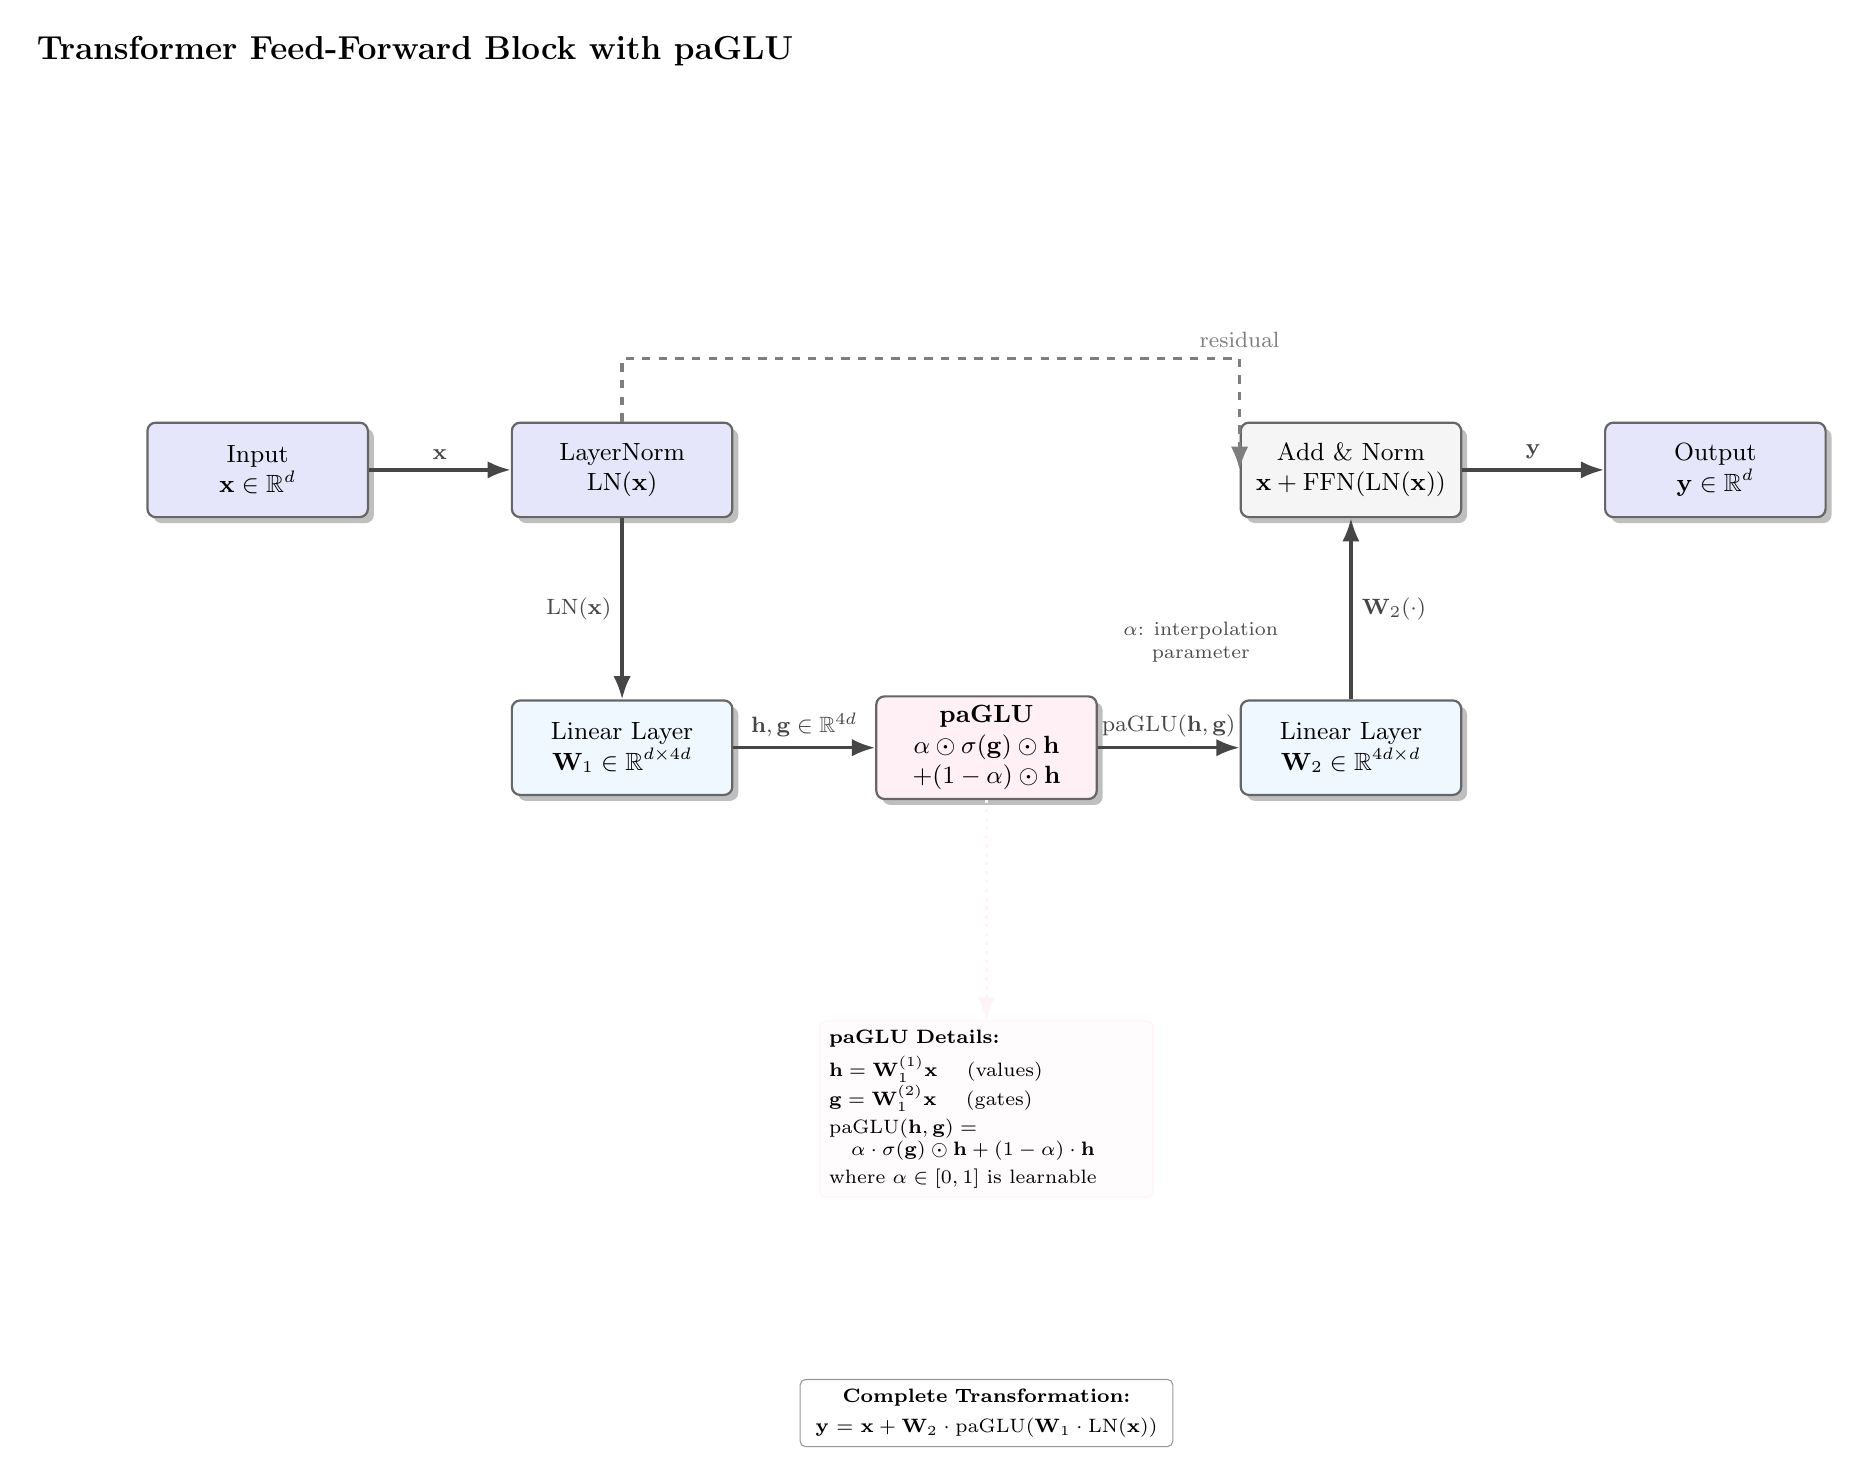
\begin{tikzpicture}[
  % Professional styling
  every node/.style={font=\small},
  block/.style={
    draw=black!60,
    rounded corners=3pt,
    minimum width=2.8cm,
    minimum height=1.2cm,
    align=center,
    line width=0.8pt,
    drop shadow
  },
  arr/.style={
    -Latex,
    thick,
    color=arrow,
    line width=1.2pt
  },
  math/.style={font=\footnotesize},
  annotation/.style={
    font=\scriptsize,
    color=black!70,
    align=center
  },
  node distance=1.8cm
]

% Title
\node[above=3cm, font=\large\bfseries] at (2,2) {Transformer Feed-Forward Block with paGLU};

% Input
\node[block, fill=layernorm] (input) at (0,0) {Input\\$\mathbf{x} \in \mathbb{R}^{d}$};

% Layer Normalization
\node[block, fill=layernorm, right=of input] (ln) {LayerNorm\\$\text{LN}(\mathbf{x})$};

% Feed Forward Components
\node[block, fill=feedforward, below=of ln, yshift=-0.5cm] (w1) {Linear Layer\\$\mathbf{W}_1 \in \mathbb{R}^{d \times 4d}$};

\node[block, fill=paglu, right=of w1] (paglu) {
  \textbf{paGLU}\\
  $\alpha \odot \sigma(\mathbf{g}) \odot \mathbf{h}$\\
  $+ (1-\alpha) \odot \mathbf{h}$
};

\node[block, fill=feedforward, right=of paglu] (w2) {Linear Layer\\$\mathbf{W}_2 \in \mathbb{R}^{4d \times d}$};

% Add & Norm (Residual)
\node[block, fill=residual, above=of w2, yshift=0.5cm] (add) {Add \& Norm\\$\mathbf{x} + \text{FFN}(\text{LN}(\mathbf{x}))$};

% Output
\node[block, fill=layernorm, right=of add] (output) {Output\\$\mathbf{y} \in \mathbb{R}^{d}$};

% Arrows with labels
\draw[arr] (input) -- (ln) node[midway,above,math] {$\mathbf{x}$};
\draw[arr] (ln) -- (w1) node[midway,left,math] {$\text{LN}(\mathbf{x})$};
\draw[arr] (w1) -- (paglu) node[midway,above,math] {$\mathbf{h}, \mathbf{g} \in \mathbb{R}^{4d}$};
\draw[arr] (paglu) -- (w2) node[midway,above,math] {$\text{paGLU}(\mathbf{h}, \mathbf{g})$};
\draw[arr] (w2) -- (add) node[midway,right,math] {$\mathbf{W}_2(\cdot)$};
\draw[arr] (add) -- (output) node[midway,above,math] {$\mathbf{y}$};

% Residual connection
\draw[arr, dashed, color=arrow!70] (ln.north) -- ++(0,0.8) -| (add.west) 
  node[midway,above,math] {residual};

% paGLU detail box
\node[
  draw=paglu!80,
  fill=paglu!20,
  rounded corners=2pt,
  below=of paglu,
  yshift=-1cm,
  text width=4cm,
  align=left,
  font=\scriptsize
] (detail) {
  \textbf{paGLU Details:}\\[2pt]
  $\mathbf{h} = \mathbf{W}_1^{(1)} \mathbf{x}$ \quad (values)\\
  $\mathbf{g} = \mathbf{W}_1^{(2)} \mathbf{x}$ \quad (gates)\\[2pt]
  $\text{paGLU}(\mathbf{h}, \mathbf{g}) = $\\
  $\quad \alpha \cdot \sigma(\mathbf{g}) \odot \mathbf{h} + (1-\alpha) \cdot \mathbf{h}$\\[2pt]
  where $\alpha \in [0,1]$ is learnable
};

% Connect detail box
\draw[arr, dotted, color=paglu!80] (paglu.south) -- (detail.north);

% Parameter annotation
\node[
  annotation,
  above right=0.3cm and 0.2cm of paglu
] {
  $\alpha$: interpolation\\
  parameter
};

% Mathematical formulation box
\node[
  draw=black!40,
  fill=white,
  rounded corners=2pt,
  below=of detail,
  yshift=-0.5cm,
  text width=4.5cm,
  align=center,
  font=\scriptsize
] (formula) {
  \textbf{Complete Transformation:}\\[3pt]
  $\mathbf{y} = \mathbf{x} + \mathbf{W}_2 \cdot \text{paGLU}(\mathbf{W}_1 \cdot \text{LN}(\mathbf{x}))$
};

\end{tikzpicture}
\end{document} 